\section{Oltre la Tree Decomposition}

L'ultima volta abbiamo visto algoritmi che avevano un $k$ fissato, avendo
complessità $\mathcal{O}(n^k)$. Ora vediamo un altro caso.

$$\mathcal{O}(n^\alpha \cdot f(k)) = \mathcal{O}(n \cdot 2^k)$$

Questi due sono rispettivamente: \textbf{Genuine Tractability} e \textbf{Fixed
    Parameter Tractability}.

\textbf{Nota:} Ricordiamo che $k$ è la width.

\subsection{Monadic Second Order Logic}
\begin{theorem}(Teorema di Courcelle)
    Sia $P$ un problema sui grafi che può essere formulato in \textbf{Monadic Second Order Logic} (MSO). Allora, il problema $P$ può
    essere risolto in tempo lineare sui grafi con \textbf{treewidth} fissata.
\end{theorem}

\begin{esempio}(3 colorabilità in MSO)
    pag 53

    \textbf{Monadic}: I predicati hanno una variabile. Sono unari.

    \textbf{Una sola relazione}: Si risolve il problema con una sola relazione. In questo caso, la relazione $E(x,y)$.
\end{esempio}

\textbf{Domanda:} Quanto è difficile impostare il problema come un grafo? E' difficile?

Pensiamo a $SAT: \exists x_,1x_2,\dots,x_n ( x_1 \lor x_2 \lor \dots \lor x_n
    ), \dots (x_1 \lor \lnot x_2 \lor \dots \lor \lnot x_n)$. Come lo portiamo ad
un grafo?

\textbf{Proposta 1:} Con una \textbf{reduction}, ma possiamo in un altro modo.

Consideriamo le $clausuole$ cioè $(x_1, \dots \lnot x_n)$ tipo. Per ogni
clausola, creiamo un nodo. Per ogni letterale, creiamo un nodo.

Ora, consideriamo 2 relazioni $edge_p(x,y)$ e $edge_n(x,y)$ che indicano valori 
\textbf{positivo} e \textbf{negativo}.

$$
    \exists T \ \forall x \ s.t. \ [(edge_p(x,\_) \lor edge_n(x,\_))] \implies \exists y edge_p(x,y) \land T(y) \lor edge_n(x,y) \land \lnot T(y)
$$

\subsection{Query Evaluation}

Quanto è complesso controllare che una query sia valida? Dipende se la query è \textbf{fissata}. Vediamo un'esempio con la \textbf{3 colorabilità}.

\begin{esempio}
    (3-COL con Query Evaluation (BCQ-EVAL))

    \begin{equation}
        \exists x,y,z,w,h r(x,y) \land r(y,z) \land r(x,w) \land r(z,w) \land r(w,h)
    \end{equation}

    E considerando un grafo
    
    \begin{figure}[H]
        \begin{center}
            \begin{tikzpicture}
                %5 nodi xyzwh
                \node[draw,circle] (x) at (0,0) {$x$};
                \node[draw,circle] (y) at (2,-2) {$y$};
                \node[draw,circle] (z) at (4,0) {$z$};
                \node[draw,circle] (w) at (2,2) {$w$};
                \node[draw,circle] (h) at (0,4) {$h$};

                \draw (x) -- (y);
                \draw (x) -- (w);
                \draw (y) -- (z);
                \draw (z) -- (w);
                \draw (w) -- (h);

            \end{tikzpicture}
        \end{center}
    \end{figure}

    \begin{table}[H]
        \begin{center}
            %tabella per relazione r con valori rg, rb, gb, ...
            \begin{tabular}{|c|c|}
                \hline
                \textbf{r} & \textbf{-} \\
                \hline
                R & G \\
                \hline 
                R & B \\
                \hline

                G & B \\
                \hline
                \dots & \dots \\
                \hline
            \end{tabular}
        \end{center}
    \end{table}
\end{esempio}

Ci sono alcuni grafi semplici che sono molto ciclici. Ad esempio, le \textbf{cricche.}
Alcuni problemi sono meglio descritti da alcune strutture dati che prendono il nome di \textbf{iper grafi}.

Consideriamo una relazione $r(x_1,x_2, \dots, x_n)$. Quanto è la treewidth? $n-1$.

Ha detto molta roba qui, ma non ho proprio capito.

\subsection{Iper grafi}

\begin{figure}[H]
    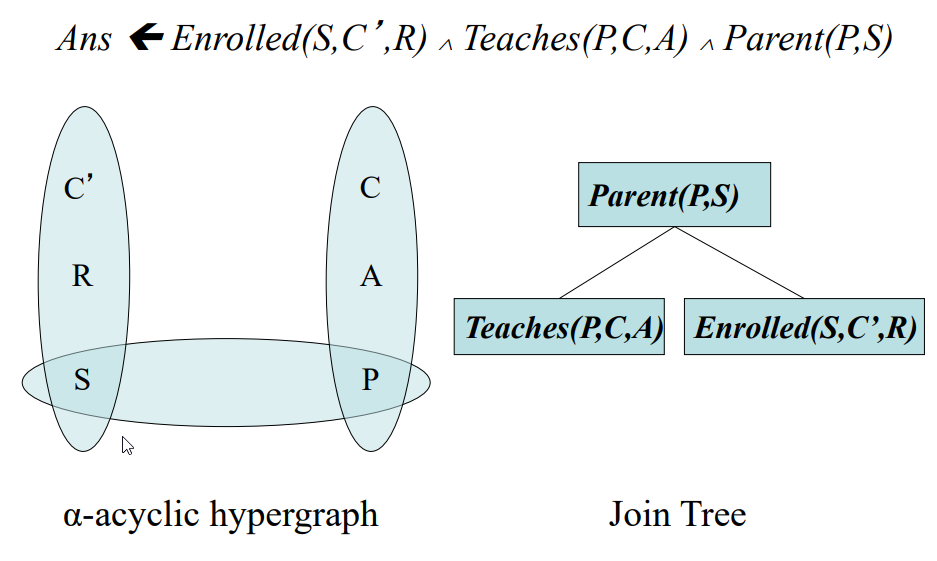
\includegraphics[scale=0.5]{chapters/images/hyper aciclic.png}
    \caption{Ipergrafo aciclico}
\end{figure}

ONestamente, di quest parte non ho capito niente e NON VOGLIO CAPIRCI NIENTE. Non si capisce niente.


\begin{esempio}
    (Applicazione di Gioco Succinto)

    A pagina 206 se vuoi leggere e provare a capire
\end{esempio}

\subsection{Problemi di Ottimizzazione}



\newpage